\documentclass[tikz,border=12pt]{standalone}
\usepackage{helvet}
\renewcommand{\familydefault}{\sfdefault}
\usepackage{tikz}
\usepackage{amsmath,amssymb}
\usetikzlibrary{positioning, fit, calc, shapes.geometric, arrows.meta, backgrounds, decorations.pathreplacing}

% Volume IV Color Palette
\definecolor{emeraldpine}{HTML}{1A4D3E}
\definecolor{harvardcrimson}{HTML}{A51C30}
\definecolor{ethdarkblue}{HTML}{1F407A}
\definecolor{ethpetrol}{HTML}{007A87}
\definecolor{ethbronze}{HTML}{B87333}
\definecolor{ethpurple}{HTML}{5B4B8A}
\definecolor{ink}{HTML}{1A202C}
\definecolor{softink}{HTML}{4A5568}
\definecolor{paleink}{HTML}{A0AEC0}
\definecolor{cardbg}{HTML}{F8FAFC}
\definecolor{panelbg}{HTML}{F1F5F9}

\begin{document}
\sffamily
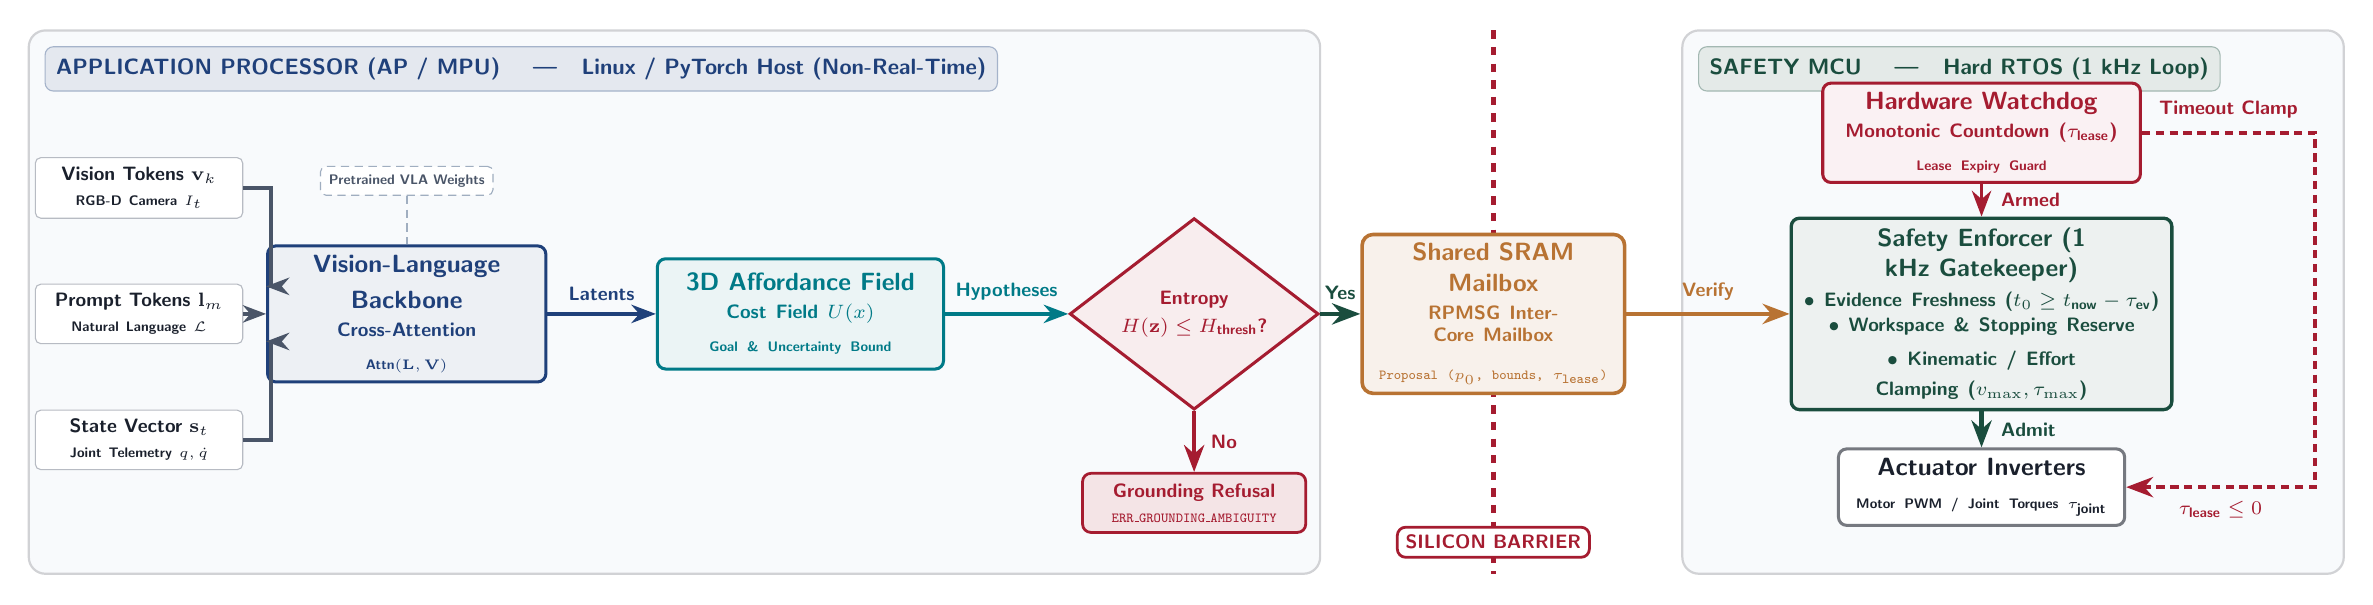
\begin{tikzpicture}[
    >=Stealth,
    font=\sffamily,
    % Node styles
    token_box/.style={draw=softink!40, fill=white, rounded corners=2pt, minimum height=0.65cm, text width=2.4cm, align=center, font=\scriptsize\bfseries, text=ink},
    proc_box/.style={draw=ethdarkblue, fill=ethdarkblue!8, rounded corners=3pt, minimum height=1.4cm, text width=3.3cm, align=center, font=\small\bfseries, text=ethdarkblue, line width=1.1pt},
    aff_box/.style={draw=ethpetrol, fill=ethpetrol!8, rounded corners=3pt, minimum height=1.4cm, text width=3.4cm, align=center, font=\small\bfseries, text=ethpetrol, line width=1.1pt},
    dia_box/.style={diamond, draw=harvardcrimson, fill=harvardcrimson!8, minimum height=1.8cm, minimum width=2.4cm, align=center, font=\scriptsize\bfseries, text=harvardcrimson, line width=1.1pt, aspect=1.3},
    refuse_box/.style={draw=harvardcrimson, fill=harvardcrimson!12, rounded corners=3pt, minimum height=0.75cm, text width=2.6cm, align=center, font=\scriptsize\bfseries, text=harvardcrimson, line width=1pt},
    sram_box/.style={draw=ethbronze, fill=ethbronze!10, rounded corners=4pt, minimum height=1.3cm, text width=3.1cm, align=center, font=\small\bfseries, text=ethbronze, line width=1.3pt},
    watch_box/.style={draw=harvardcrimson, fill=harvardcrimson!6, rounded corners=3pt, minimum height=1.2cm, text width=3.8cm, align=center, font=\small\bfseries, text=harvardcrimson, line width=1.1pt},
    safe_box/.style={draw=emeraldpine, fill=emeraldpine!8, rounded corners=3pt, minimum height=1.6cm, text width=4.6cm, align=center, font=\small\bfseries, text=emeraldpine, line width=1.2pt},
    act_box/.style={draw=ink!60, fill=white, rounded corners=3pt, minimum height=0.85cm, text width=3.4cm, align=center, font=\small\bfseries, text=ink, line width=1.1pt},
]

    % =========================================================
    % 1. APPLICATION PROCESSOR (AP / MPU) DOMAIN
    % =========================================================
    % Background Container Box
    \filldraw[fill=cardbg, draw=ink!20, rounded corners=6pt, line width=0.8pt] 
      (-1.8, -3.3) rectangle (14.6, 3.6);
    
    % Domain Header Badge
    \node[fill=ethdarkblue!12, draw=ethdarkblue!40, rounded corners=3pt, font=\bfseries\footnotesize, text=ethdarkblue, anchor=north west, inner sep=4pt] 
      at (-1.6, 3.4) {APPLICATION PROCESSOR (AP / MPU) \quad \textemdash \quad Linux / PyTorch Host (Non-Real-Time)};

    % Multimodal Inputs & Tokens
    \node[token_box] (tok_vis) at (-0.4, 1.6) {
      \textbf{Vision Tokens $\mathbf{v}_k$}\\[1pt]
      \tiny RGB-D Camera $I_t$
    };
    \node[token_box] (tok_pmt) at (-0.4, 0.0) {
      \textbf{Prompt Tokens $\mathbf{l}_m$}\\[1pt]
      \tiny Natural Language $\mathcal{L}$
    };
    \node[token_box] (tok_st) at (-0.4, -1.6) {
      \textbf{State Vector $\mathbf{s}_t$}\\[1pt]
      \tiny Joint Telemetry $q, \dot{q}$
    };

    % Multi-Modal Cross-Attention / VLA Backbone
    \node[proc_box] (vla) at (3.0, 0.0) {
      \textbf{Vision-Language}\\[2pt]
      \textbf{Backbone}\\[2pt]
      \scriptsize Cross-Attention\\[1pt]
      \tiny $\text{Attn}(\mathbf{L}, \mathbf{V})$
    };

    % Pretrained Foundation Weights Callout
    \node[draw=paleink, fill=white, rounded corners=2pt, inner sep=3pt, font=\tiny\bfseries, text=softink, densely dashed, anchor=south] 
      (pre) at (3.0, 1.5) {Pretrained VLA Weights};
    \draw[densely dashed, paleink, thick] (pre.south) -- (vla.north);

    % 3D Affordance Cost Field Generator
    \node[aff_box] (aff) at (8.0, 0.0) {
      \textbf{3D Affordance Field}\\[2pt]
      \scriptsize Cost Field $U(x)$\\[1pt]
      \tiny Goal \& Uncertainty Bound
    };

    % Producer-side Entropy Gate
    \node[dia_box] (dia) at (13.0, 0.0) {
      \textbf{Entropy}\\[2pt]
      $H(\mathbf{z}) \le H_{\text{thresh}}$?
    };

    % Ambiguity Refusal Response
    \node[refuse_box] (refuse) at (13.0, -2.4) {
      \textbf{Grounding Refusal}\\[1pt]
      \tiny \texttt{ERR\_GROUNDING\_AMBIGUITY}
    };

    % Connectors inside AP
    \draw[->, line width=1.2pt, softink] (tok_vis.east) -- ++(0.35, 0) |- ($(vla.west) + (0, 0.35)$);
    \draw[->, line width=1.2pt, softink] (tok_pmt.east) -- (vla.west);
    \draw[->, line width=1.2pt, softink] (tok_st.east)  -- ++(0.35, 0) |- ($(vla.west) + (0, -0.35)$);

    \draw[->, line width=1.3pt, ethdarkblue] (vla.east) -- node[above, font=\scriptsize\bfseries, text=ethdarkblue, yshift=1pt] {Latents} (aff.west);
    \draw[->, line width=1.3pt, ethpetrol] (aff.east) -- node[above, font=\scriptsize\bfseries, text=ethpetrol, yshift=1pt] {Hypotheses} (dia.west);

    \draw[->, line width=1.5pt, harvardcrimson] (dia.south) -- node[right, font=\bfseries\scriptsize, text=harvardcrimson, xshift=2pt] {No} (refuse.north);

    % =========================================================
    % 2. INTER-CORE SILICON BOUNDARY & SHARED SRAM
    % =========================================================
    \def\xBarrier{16.8}

    % Silicon Barrier Vertical Separator
    \draw[dashed, harvardcrimson, line width=2pt] (\xBarrier, 3.6) -- (\xBarrier, 0.95);
    \draw[dashed, harvardcrimson, line width=2pt] (\xBarrier, -0.95) -- (\xBarrier, -3.3);
    
    \node[fill=white, draw=harvardcrimson, rounded corners=3pt, font=\bfseries\scriptsize, text=harvardcrimson, inner sep=3pt, line width=1pt] 
      at (\xBarrier, -2.9) {SILICON BARRIER};

    % Shared Memory Mailbox (Bridging AP and MCU)
    \node[sram_box] (sram) at (\xBarrier, 0.0) {
      \textbf{Shared SRAM Mailbox}\\[2pt]
      \scriptsize RPMSG Inter-Core Mailbox\\[3pt]
      \tiny \ttfamily Proposal ($p_0$, bounds, $\tau_{\text{lease}}$)
    };

    % Admission into Shared SRAM
    \draw[->, line width=1.6pt, emeraldpine] (dia.east) -- node[above, font=\bfseries\scriptsize, text=emeraldpine, yshift=1pt] {Yes} (sram.west);

    % =========================================================
    % 3. REAL-TIME SAFETY MCU DOMAIN
    % =========================================================
    % Background Container Box
    \filldraw[fill=cardbg, draw=ink!20, rounded corners=6pt, line width=0.8pt] 
      (19.2, -3.3) rectangle (27.6, 3.6);

    % Domain Header Badge
    \node[fill=emeraldpine!12, draw=emeraldpine!40, rounded corners=3pt, font=\bfseries\footnotesize, text=emeraldpine, anchor=north west, inner sep=4pt] 
      at (19.4, 3.4) {SAFETY MCU \quad \textemdash \quad Hard RTOS (1 kHz Loop)};

    % Hardware Watchdog / Lease Countdown Timer
    \node[watch_box] (watch) at (23.0, 2.3) {
      \textbf{Hardware Watchdog}\\[2pt]
      \scriptsize Monotonic Countdown ($\tau_{\text{lease}}$)\\[1pt]
      \tiny Lease Expiry Guard
    };

    % Real-Time Safety Enforcer (Spatial-Temporal Bounds Checker)
    \node[safe_box] (safe) at (23.0, 0.0) {
      \textbf{Safety Enforcer (1 kHz Gatekeeper)}\\[3pt]
      \scriptsize $\bullet$ Evidence Freshness ($t_0 \ge t_{\text{now}} - \tau_{\text{ev}}$)\\[1pt]
      \scriptsize $\bullet$ Workspace \& Stopping Reserve\\[1pt]
      \scriptsize $\bullet$ Kinematic / Effort Clamping ($v_{\max}, \tau_{\max}$)
    };

    % Actuator Inverters
    \node[act_box] (act) at (23.0, -2.2) {
      \textbf{Actuator Inverters}\\[1pt]
      \tiny Motor PWM / Joint Torques $\tau_{\text{joint}}$
    };

    % Connectors in MCU
    \draw[->, line width=1.5pt, ethbronze] (sram.east) -- node[above, font=\scriptsize\bfseries, text=ethbronze, yshift=1pt] {Verify} (safe.west);
    \draw[->, line width=1.4pt, harvardcrimson] (watch.south) -- node[right, font=\scriptsize\bfseries, text=harvardcrimson, xshift=3pt] {Armed} (safe.north);
    \draw[->, line width=1.5pt, emeraldpine] (safe.south) -- node[right, font=\bfseries\scriptsize, text=emeraldpine, xshift=3pt] {Admit} (act.north);

    % Timeout Clamp / Revocation Path (Direct Hardware Clamp to Actuators)
    \draw[->, harvardcrimson, line width=1.5pt, densely dashed] 
      (watch.east) -- node[above, font=\scriptsize\bfseries, text=harvardcrimson, yshift=1pt] {Timeout Clamp} ++(2.2, 0) coordinate (c_top) 
      -- (c_top |- act.east) 
      -- node[below, font=\scriptsize\bfseries, text=harvardcrimson, yshift=-1pt] {$\tau_{\text{lease}} \le 0$} (act.east);

\end{tikzpicture}
\end{document}
